\documentclass[12pt,a4paper,titlepage,openany]{report}
\usepackage{zakljucna_FAMNIT_1_stopnja_MA_MEF_EN_2016}
\usepackage{subcaption}
\graphicspath{ {./images/} }


% Head of document:

\fancyhf{}
\lhead[]{{\fontsize{9.3}{12}\selectfont
Convolutional neural network for eyeblink artifact detection in EEG data.\\
\noindent Univerza na Primorskem, Fakulteta za matematiko, naravoslovje in informacijske tehnologije, 2025}}
\chead[]{\fancyplain{}{}}
\rhead[]{\fancyplain{\thepage}
{\thepage}}
\cfoot[]{\fancyplain{}{}}
\lfoot[]{\fancyplain{}{}}
\rfoot[]{\fancyplain{}{}}
\normalsize

%%%%%%%%%%%%%%%%%%%%%%%%% BEGINNING OF DOCUMENT %%%%%%%%%%%%%%%%%%%%%%%%%%%%%%%%%%%%%%%%%%5

%%%%%%%%%%%%%%%%%%%%%%%%% Title page %%%%%%%%%%%%%%%%%%%%%%%%%


\begin{document}
\pagenumbering{Roman}
\pagestyle{empty}
\begin{center}
\noindent \large UNIVERZA NA PRIMORSKEM\\
\large FAKULTETA ZA MATEMATIKO, NARAVOSLOVJE IN\\
INFORMACIJSKE TEHNOLOGIJE


\normalsize
\vspace{5.5cm}
Zaklju\v cna naloga\\
(Final project paper)\\
\textbf{\large Naslov zaklju\v cne naloge}\\
\normalsize
(Convolutional neural network for eyeblink artifact detection in EEG data)\\
\end{center}

\begin{flushleft}
\vspace{5cm}
\noindent Ime in priimek: Marko Jankovic
% add your first name and last name in the line above
\\
\noindent \v Studijski program: (name of the study program, in Slovene)
% add your study program in the line above
\\
\noindent Mentor: (with all titles, in Slovene)
% add the academic title, first name, and last name of your mentor in the line above
\\
\noindent Somentor: (with all titles, in Slovene)
% if you have a co-mentor, add his/her academic title, first name, and last name in the line above
% if you do not have a co-mentor, delete the line above and the line below
\\
\end{flushleft}

\vspace{4cm}
\begin{center}
\large \textbf{Koper, mesec leto}
% add the month and year of submission of your final project paper
\end{center}
\newpage

\pagestyle{fancy}
%%%%%%%%%%%%%%%%%%%%%%%%%%%%%%% Key words documentation (Slovene and English) %%%%%%%%%%%

\section*{Klju\v cna dokumentacijska informacija}

\medskip
\begin{center}
\fbox{\parbox{\linewidth}{
\vspace{0.2cm}
\noindent
Ime in PRIIMEK: Marko Jankovic \vspace{0.5cm}\\
Naslov zaklju\v cne naloge:\vspace{0.5cm}\\
Kraj: Koper\vspace{0.5cm}\\
Leto: 2025 \vspace{0.5cm}\\
\v Stevilo listov: \hspace{2cm} \v Stevilo slik: \hspace{2.6cm} \v Stevilo tabel:\hspace{2cm}\vspace{0.5cm}\\
\v Stevilo prilog: \hspace{1.9cm} \v Stevilo strani prilog: \hspace{1cm} \v Stevilo referenc:\vspace{0.5cm}\\
Mentor:\vspace{0.5cm}\\
Somentor:\vspace{0.5cm}\\
Klju\v cne besede:\vspace{0.5cm}\\
Math.~Subj.~Class.~(2010):\vspace{0.5cm}\\
{\bf Izvle\v cek:}\\
Izvle\v cek predstavlja kratek, a jedrnat prikaz vsebine naloge. V najve\v c 250 besedah nakažemo problem, metode, rezultate, klju\v cne ugotovitve in njihov pomen.
\vspace{0.2cm}
}}
\end{center}

\newpage

\section*{Key words documentation}

\medskip

\begin{center}
\fbox{\parbox{\linewidth}{
\vspace{0.2cm}
\noindent
Name and SURNAME: Marko Jankovic\vspace{0.5cm}\\
Title of final project paper: Convolutional neural network for eyeblink artifact detection in EEG data\vspace{0.5cm}\\
Place: Koper \vspace{0.5cm}\\
Year: 2025\vspace{0.5cm}\\
Number of pages:\hspace{1.6cm} Number of figures:\hspace{2.2cm} Number of tables:\vspace{0.5cm}\\
Number of appendices:\hspace{0.6cm} Number of appendix pages:\hspace{0.8cm}Number of references:\vspace{0.5cm}\\
Mentor: title~First Name~Last Name, PhD\vspace{0.5cm}\\
% for : "title" write one of the following:
% Assist.~Prof.~(if the title is "docent"),
% Assoc.~Prof.~(if the title is "izredni profesor"),
% Prof.~(if the title is "profesor")
Co-Mentor:\vspace{0.5cm}\\
Keywords:\vspace{0.5cm}\\
Math.~Subj.~Class.~(2010):\vspace{0.5cm}\\
{\bf Abstract:}
\vspace{0.2cm}
}}
\end{center}




%%%%%%%%%%%%%%%%%%%%%%%%%%%%%%% Acknowledgement %%%%%%%%%%%%%%%%%%%%%%%%%%%%%%%%%%%%%

\newpage
\section*{Acknowledgement}

Here we thank all involved with our final project paper, that is, persons or institutions that helped us in our work and/or made it possible.
We can also thank the mentor and the co-mentor (if there is one).

%%%%%%%%%%%%%%%%%%%%%%%%%%%%% Table of contents, list of figures, etc. %%%%%%%%%%%%%%%%%%%%%%%%%%%%%%
\newpage

\tableofcontents
\addtocontents{toc}{\protect\thispagestyle{fancy}}
% if there are no tables in your final project paper, delete the following three lines
\newpage
\listoftables
\addtocontents{lot}{\protect\thispagestyle{fancy}}
% if there are no figures in your final project paper, delete the following three lines
\newpage
\listoffigures
\addtocontents{lof}{\protect\thispagestyle{fancy}}
\newpage
% Since the appendices are not numbered, we also do not want to show the dots to their (non-existing) page numbers.
\renewcommand{\cftdot}{}
\listofappendices{}
\thispagestyle{fancy}
\newpage

\chapter*{List of Abbreviations}
\thispagestyle{fancyplain}
\begin{longtable}{@{}p{1cm}@{}p{\dimexpr\textwidth-1cm\relax}@{}}
\nomenclature{{\it i.e.}}{that is}
\nomenclature{{\it e.g.}}{for example}
\end{longtable}
\newpage

\normalsize

%%%%%%%%%%%%%%%%%%%%%%%%%%%%%%%%%% Chapters: %%%%%%%%%%%%%%%%%%%%%%%%%%%%%%%%%%%%%

% Hint: You might find it convenient to keep the contents of separate chapters in separate files, each in their own
% .tex file. They all have to be stored in the same folder as the main file. Each chapter is included with the \include command.
% Example: we can insert FirstChapter.tex and SecondChapter.tex as follows:
% \include{FirstChapter}
% \include{SecondChapter}

%%%%%%%%%%%%%%%%%%%%%%%%%%%%%%%%%% Chapter 1: Introduction %%%%%%%%%%%%%%%%%%%%%%%%%%%%%%%%%%%%%


\chapter{Introduction}
\thispagestyle{fancy}
\pagenumbering{arabic}

Electroencephalogram (EEG) is a noninvasive neuroimaging technique that involves the placement of electrodes on the scalp to record the electrical activity of the brain. This enables researchers to measure and analyze the electrical signals generated by the brain. These signals offer valuable information on the operating mechanisms of the brain, covering the identification of various neurological disorders and the exploration of cognitive processes such as perception, attention, and memory.
However, EEG signals are prone to various artifacts, one of the most frequent being eye blinks, which for adults typically occur 15-20 times per minute. Eye closure changes brain activity, so eye-blink tracking of subjects undergoing EEG analysis is relevant for identifying when a subject blinks, falls asleep, or keeps their eyes closed. 
Eye blink and muscle movement artifacts are usually unwanted signals in the brain that can contaminate EEG data significantly and affect the accuracy of subsequent analysis of brain activity that is being measured with an electroencephalogram (EEG). 
Traditional methods for detecting and removing eye blink artifacts involve manual inspection, filtering, or statistical techniques like Independent Component Analysis (ICA). While these methods can work, they are very time-consuming and prone to human error, especially in real-time applications. They also fail to capture the complex spatial and temporal relationships in EEG data, hence they vary for different subjects and recording conditions.

\section{Purpose of the thesis}

In recent years CNNs have shown to be very effective in various domains as they can learn hierarchical features from raw data. 
This thesis proposes a CNN-based approach to detect signals in EEG data automatically, by demonstrating this ability on detection of eye blink artifacts. 
The aim is to design a model to detect signals in EEG recordings and with that prove that neural networks can be used to enhance EEG recordings and make EEG-based systems perform better.

%%%%%%%%%%%%%%%%%%%%%%%%%%%%%%%%%% Chapter 2: Background and context %%%%%%%%%%%%%%%%%%%%%%%%%%%%%%%%%%%%%

\chapter{Background and context}
\thispagestyle{fancy}

\section{Electroencephalography (EEG)}

Electroencephalography (EEG) is the measurement of the electric potentials on the scalp surface generated (in part) by neural activity originating from the brain. 
The sensitivity of EEG to changes in brain activity on such a millisecond time scale is the major advantage of EEG over other brain imaging modalities such as functional magnetic resonance imaging (fMRI) or near-infrared spectroscopy (NIRS) that operate on time scales in the seconds to minutes range. 
Over the past 100 years, neuroscientists and clinical neurologists have made use of EEG to obtain insight into cognitive or clinical disease state by applying a variety of signal processing and statistical analyses to EEG time series. 
More recently there has been growing interest in making use of statistical modeling of EEG signals to directly control physical devices in Brain-Computer Interfaces.
EEG power is typically split up into bands which correspond to different spectral peaks that relate to behavior or cognitive state. These bands are typically defined as the delta (1-4 Hz), theta (4-8 Hz), alpha (8-13 Hz), beta (13-20 Hz), and gamma (\textgreater 20 Hz).\cite{nunez2016}

\section{Neural Networks}

Convolutional networks have been applied to sequences for decades. They were used prominently for speech recognition in the 80s and 90s. 
ConvNets were subsequently applied to NLP tasks such as part-of-speech tagging and semantic role labelling. 
More recently, convolutional networks were applied to sentence classification and document classification. 
Recurrent networks are dedicated sequence models that maintain a vector of hidden activations that are propagated through time. 
This family of architectures has gained tremendous popularity due to prominent applications to language modeling and machine translation. 
The intuitive appeal of recurrent modeling is that the hidden state can act as a representation of everything that has been seen so far in the sequence. 
Basic RNN architectures are notoriously difficult to train and more elaborate architectures are commonly used instead, such as the LSTM and the GRU. 
Many other architectural innovations and training techniques for recurrent networks have been introduced and continue to be actively explored.
Other recent works have aimed to combine aspects of RNN and CNN architectures. This includes the Convolutional LSTM, which replaces the fully-connected layers in an LSTM with convolutional layers to allow for additional structure in the recurrent layers; the Quasi-RNN model that interleaves convolutional layers with simple recurrent layers; and the dilated RNN, which adds dilations to recurrent architectures.\\

First, we describe a generic architecture for convolutional sequence prediction. 
The aim is to distill the best practices in convolutional network design into a simple architecture that can serve as a convenient but powerful starting point. 
The presented architecture is referred to as a temporal convolutional network (TCN), emphasizing that this term serves not as a label for a truly new architecture, but as a simple descriptive term for a family of architectures. 
The distinguishing characteristics of TCNs are: 
\begin{enumerate}
     \item the convolutions in the architecture are causal, meaning that there is no information “leakage” from future to past; 
     \item the architecture can take a sequence of any length and map it to an output sequence of the same length, just as with an RNN. 
\end{enumerate}   
Beyond this, it is emphasized how to build very long effective history sizes (i.e., the ability for the networks to look very far into the past to make a prediction) using a combination of very deep networks (augmented with residual layers) and dilated convolutions. The architecture is informed by recent convolutional architectures for sequential data, but is distinct from all of them and was designed from first principles to combine simplicity, autoregressive prediction, and very long memory. For example, the TCN is much simpler than WaveNet (no skip connections across layers, conditioning, context stacking, or gated activations). 
Compared to the other language modeling architectures, TCNs do not use gating mechanisms and have much longer memory.\cite{bai2018}

\section{ICA label}

ICA was firstly created for dealing with the cocktail party problem, upon which you attempt to isolate a pertinent conversation from the noise of other conversations in a cocktail party. Applying the ICA to the EEG data involves the decomposition of EEG time series data into a set of components. More specifically, EEG data are transformed to a collection of simultaneously recorded outputs of spatial filters applied to the whole multi-channel data, instead of a collection of simultaneously recorded single-channel data records. Thus, ICA is also a source separation technique that attempts to identify independent sources of variance in the EEG data. 
In the original EEG data collected at single channels, each row of the recording data matrix represents the time course of summed in voltage differences between the respective channel and the references channels. 
After ICA decomposition, each row of the transformed data matrix represents the time course of the activity of one independent component that is spatially filtered from the channel data. 
The outputs of ICA procedure are statistically independent component (IC) waveforms, as well as matrix that transforms EEG data to IC data, and its inverse matrix to transform IC data back to EEG data. 
These outputs provide information about an IC’s temporal and spatial properties. Concerning that ICA assumes an instantaneous relationship (e.g., common volume conduction) and that any relationship between EEG and EMG signals should involve propagation delays, it is recommended to only select EEG channels for ICA decomposition.\cite{makkar2023}

\subsection{ICA label based artifact removal}

The EEG data recorded from scalp electrodes can be considered summations of real EEG signals and artifacts, which are independent of each other. ICA is therefore potentially a useful methodology to separate artifacts from EEG signals. To removal artifacts embedded in EEG recordings, the computed ICs are firstly classified as either artefactual or neural related components. If detected and flagged as artifact-related ICs, they can be subtracted from the recorded data, and the remaining data can be remixed. In the artifact correction, ICA is used to separate components in order to identify artifacts relevant with eye movements or heartbeats. 
These relevant ICs have characteristic shapes (topographies, time courses, and frequency spectra) and can often be identified automatically. 
That is, artifact-relevant components generally can be identified according to the topographies, across-trial temporal distributions, and frequency distributions of the components. 

Abnormal topographies can be appeared as (1) power concentrated only in the frontal lobe in topography (ocular artifacts); (2) discontinued topography (noise artifacts); and (3) topography constrained within single electrode (electrode artifacts). 
Abnormal across-trial temporal distributions can be appeared as (1) inconsistent between epochs (without obvious peaks in average waveforms); (2) periodic waveform (power line interference); and (3) noisy pattern (similar to Gaussian noise). 
In addition, the frequency of artifact relevant components is in higher-frequency band (e.g., \textgreater 30 Hz), while the frequency content of neural signals is in lower-frequency band (e.g., 5–20 Hz). 
Particularly, for components relevant with blink artifacts (as shown in Fig. \ref{fig:ICA}), they have an anterior distribution, and their time courses are largely flat with occasional very high-amplitude spikes indicating artifacts of the eye muscles as they close and open.

\begin{figure}[h]
     \centering
     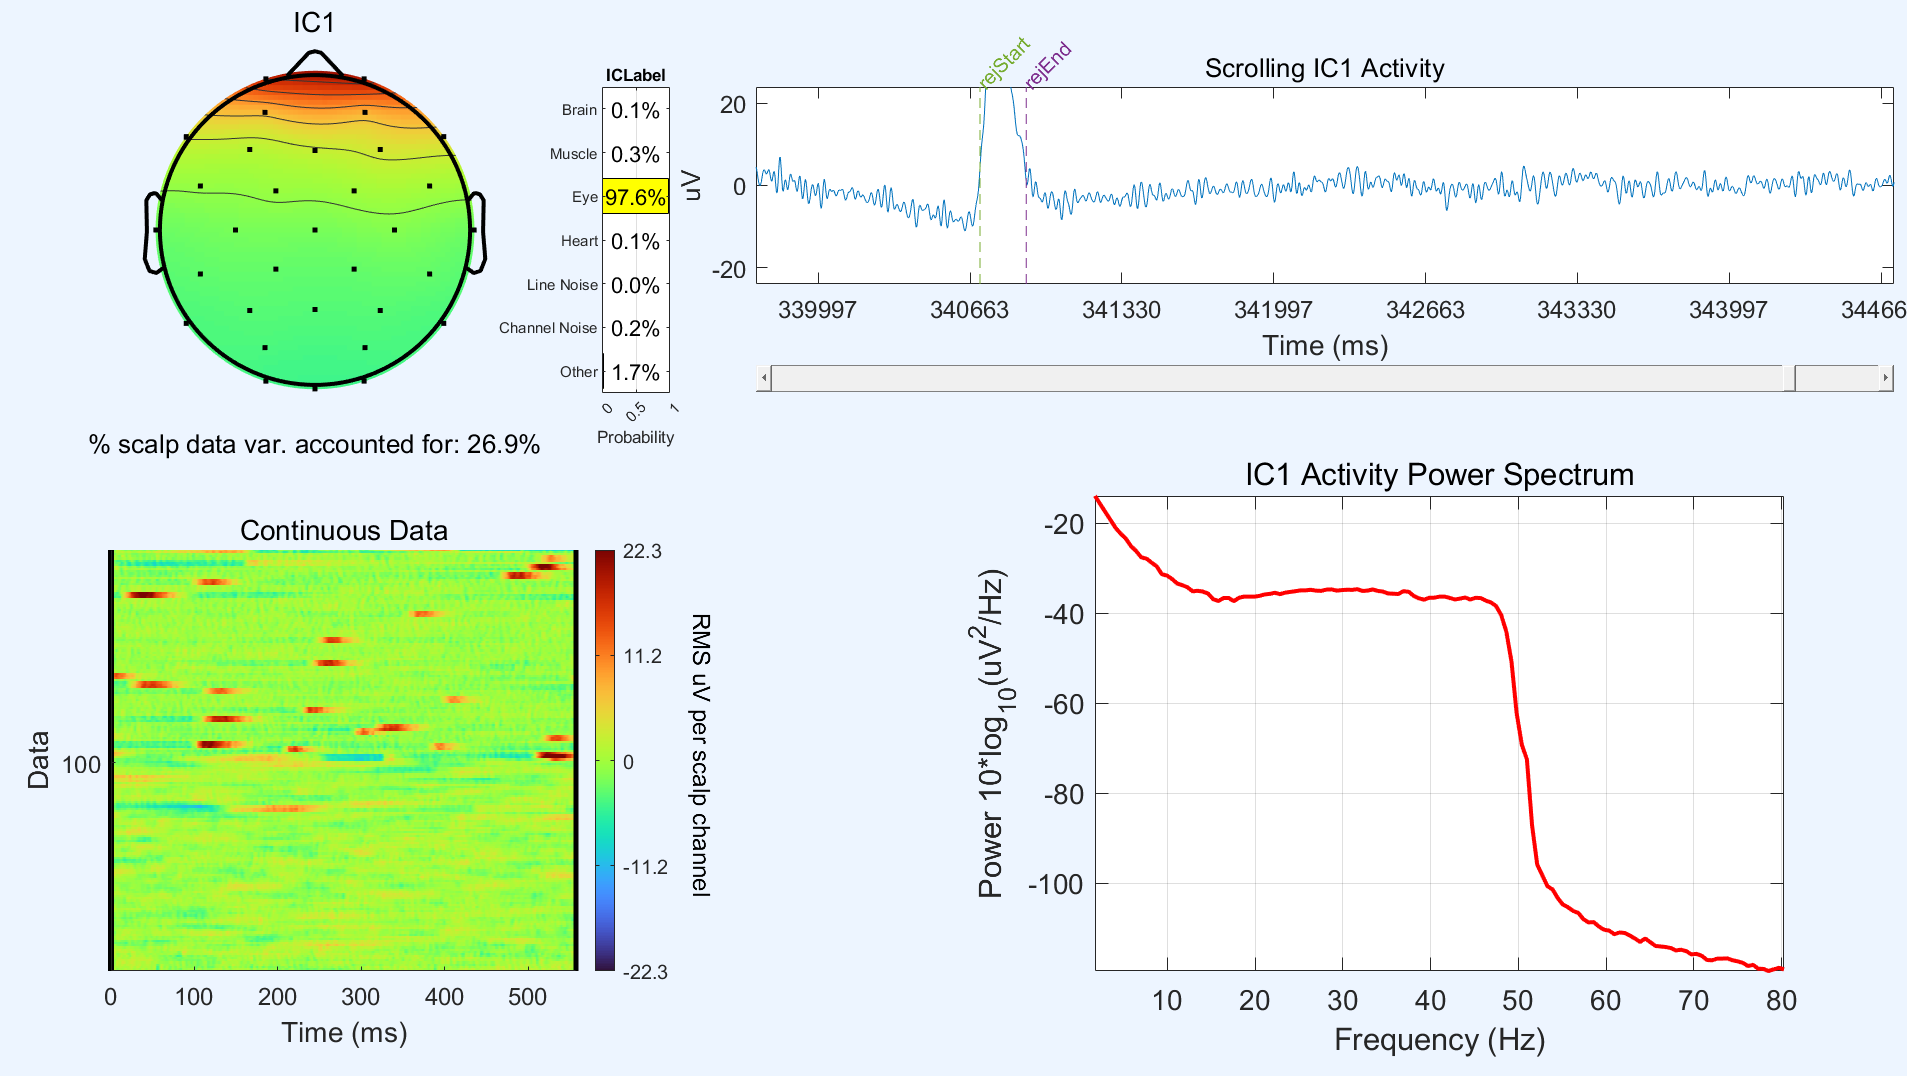
\includegraphics[scale=0.5]{./Chapter3_Methodology/Eye-blink via ICA label.png}
     \caption{Examples of components relevant with ocular artifacts.}
     \label{fig:ICA}
\end{figure}

Particularly, the application of ICA seems to be particularly useful in removing blinks and other oculomotor artifacts. Using ICA to correct artifacts is generally considered the best, since it does not assume orthogonal or gaussian behavior of the individual signals. 
In contrast, PCA (principal component analysis) assumes that all signals are orthogonal and creates a succession of orthogonal base vectors, where each vector will account for as much variance as possible. 
As a result, the first vector from PCA is significantly larger in magnitude than all the subsequent vectors. 
When the signal to noise ratio is low, important information in these subsequent vectors can get lost.\cite{makkar2023}

%%%%%%%%%%%%%%%%%%%%%%%%%%%%%%%%%% Chapter 3: Methodology %%%%%%%%%%%%%%%%%%%%%%%%%%%%%%%%%%%%%


\chapter{Methodology}
\thispagestyle{fancy}

In this section, the proposed methodology is described stepwise. First, a description of the data is given, and then the data pre-processing is explained, followed by the architecture of the model.

\section{Datasets}

\subsection{Datasets description}

This dataset examines the effects of caffeine on brain stimulation and consists of EEG recordings of two categories of participants: the first group which had an intake of regular coffee, and the other which had decaffeinated coffee. 
The primary difference between the two types of participants was the drinks and hence caffeine content. 
Participants from both groups were given the chance to add different amounts of sugar to their drinks, which causes an issue with the data but this is not the concern of this analysis.

In relation to our project, this dataset will be used for dealing with artifact identification and detection in EEG data, and while the original research was focused on caffeine stimulation of the brain, we are interested only in artifacts present in EEG signals, such as blinking, movements of muscles, and other activities nearby that interfere with the EEG readings.

\subsection{Data preprocessing}

While EEG recordings tend to contain noise and artifacts such as eye blinking or movement, EEG signals measured from the scalp do not necessarily accurately represent signals originating from the brain. 
Therefore, it is very essential to apply preprocessing and denoising to the recorded EEG data. 
Generally, preprocessing steps include the transformations or reorganizations of the recorded EEG data by removing bad or artifact-ridden data without changing clean data (transformation) and segmenting continuous raw signals without change of the data (reorganizations).

Our preprocessing of the data comes in 6 steps:

\begin{enumerate}
    \item Filter 1 to 50Hz:
    
    We apply a bandpass filter to the EEG data, keeping frequencies between 1 Hz (lower limit) and 50 Hz (upper limit).

    1 Hz: This high-pass filter removes very slow components (below 1 Hz) that may correspond to artifacts like slow drifts in signals.

    50 Hz: This low-pass filter removes fast components above 50 Hz, such as muscle artifacts and electrical noise.

    \item Cutaway first 1000 samples

    We remove the first 1000 samples, which might correspond to initial noise or artifacts at the start of the recording. 

    \item Re-reference to average

    This step re-references the EEG signals by subtracting the average of all electrodes from each electrode. This is commonly done to minimize noise and make the signals more comparable across channels.

    The assumption of average reference is: the sum of the electric field values recorded at all scalp electrodes (sufficiently dense and evenly distributed) is always 0, and the current passing through the base of the skull to the neck and body is negligible. 
    Since our EEG recording system has enough even channels using average reference makes sense as the overall activity averages to 0.

    \item Resample from 600 to 300 Hz

    We resample the data from a sampling rate of 600 Hz to 300 Hz. Resampling reduces the data size while retaining enough frequency resolution for EEG analysis.

    \item Check dataset integrity

    This function checks the integrity of the EEG dataset after the preprocessing steps to ensure there are no inconsistencies or issues.

    \item Run ICA

    In this step, Independent Component Analysis (ICA) is applied to separate independent sources (e.g., eye blinks, muscle noise, and brain activity) in the EEG signals. This helps in identifying and later removing artifacts, which is a common step after the basic preprocessing (filtering, re-referencing, etc.) has been completed.

\end{enumerate}

\section{Model selection and description}

%%%%%%%%%%%%%%%%%%%%%%%%%%%%%%%%%% Chapter 4: Results %%%%%%%%%%%%%%%%%%%%%%%%%%%%%%%%%%%%%

\chapter{Results}
\thispagestyle{fancy}

In this chapter, we report the performance of our model using key metrics such as accuracy, precision, and recall. These results show how well the model identifies and classifies artifacts in our test dataset.
We will examine the results of our thorough testing process. The outcomes of our model's tests, both qualitative and quantitative, are presented here in our analysis. In addition to highlighting the model's potential, this assessment points out the drawbacks or areas in need of more development.

\section{Results of training}

The training process was done on two datasets, with an already established model architecture without any modifications to its structure or hyperparameters. The focus of this training was replicating the performance suggested in previous studies, and using it to prove our hypothesis. 
As a result, no validation dataset was included in the training phase, and the choice was made based on lack of changes to the model that would require additional validation. \\

In Fig. \ref{fig:training} we display the accuracy and loss training measures. 
Within the first few epochs, the model achieves nearly perfect training accuracy, indicating rapid convergence of the accuracy curve.
Also we can see this in the training loss curve, where we observe steep decline during the initial iterations and in the further training it stabilizes at minimal values.
This demonstrates the model's ability to successfully fit the training data and is consistent with our expectations of it.

\begin{figure}[h]
     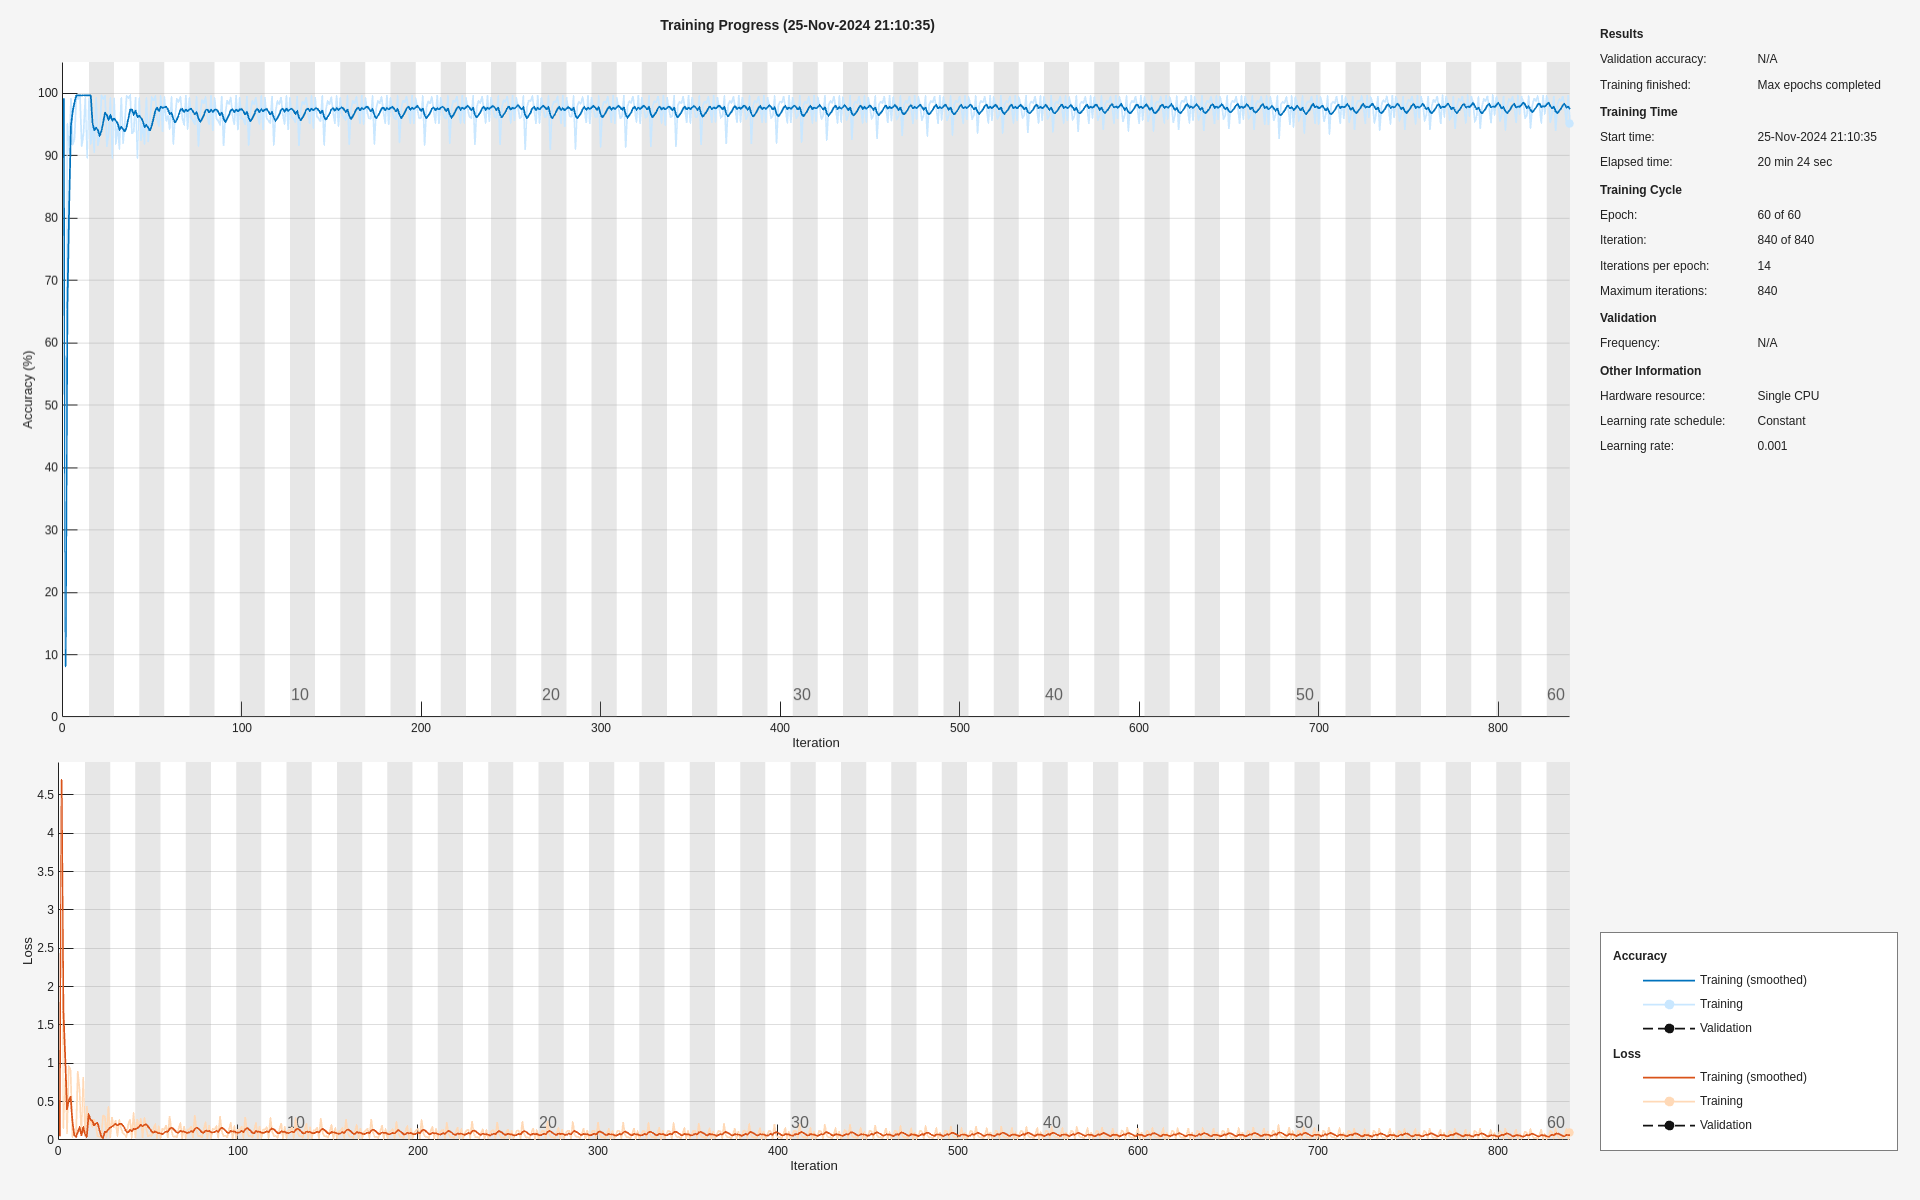
\includegraphics[scale=0.5]{./new_training/training_chart_new.png}
     \caption{Results of training}
     \label{fig:training}
\end{figure}

\section{Results of testing the model}

Here we present the results of testing our model.

     \begin{figure}[h]
          \begin{subfigure}{0.5\textwidth}
          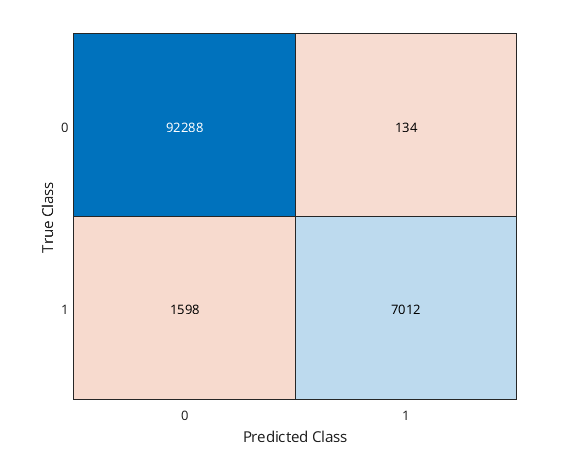
\includegraphics[scale=0.5]{./new_training/training_test_data_confusion_chart_new.png}
          \caption{Confusion matrix}
          \end{subfigure}
          \begin{subfigure}{0.5\textwidth}
          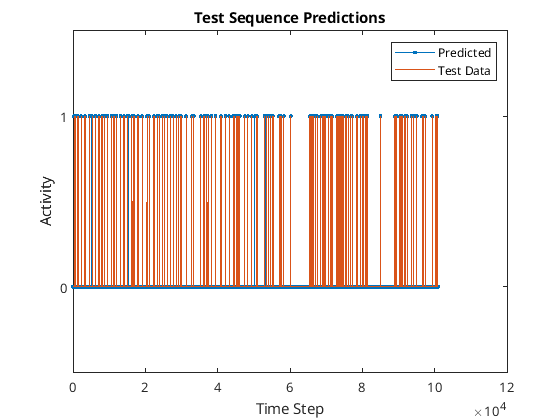
\includegraphics[scale=0.5]{./new_training/test_sequence_predictions_new.png}
          \caption{Time-series line chart}
          \end{subfigure}
     \caption{Results of testing}
     \end{figure}

\section{Alternative model comparisson}


ddddd


%%%%%%%%%%%%%%%%%%%%%%%%%%%%%%%%%% Chapter 5: Discussion and conclusion %%%%%%%%%%%%%%%%%%%%%%%%%%%%%%%%%%%%%


\chapter{Discussion and conclusion}
\thispagestyle{fancy}

In few sentences we briefly summarize the content of the project paper.
This is also the place where we can add some further references for the interested reader.

%%%%%%%%%%%%%%%%%%%%%%%%%%%%%%%%%% Chapter 6: Literature %%%%%%%%%%%%%%%%%%%%%%%%%%%%%%%%%%%%%

\begin{thebibliography}{99}
\thispagestyle{fancy}
     
\bibitem{nunez2016}
     Michael Nunez, Paul Nunez, and Ramesh Srinivasan, 
     \emph{Electroencephalography (EEG): Neurophysics, Experimental Methods, and Signal Processing}, 
     Jan. 1, 2016, pp. 175--197, ISBN: 978-1-4822-2097-1, DOI: \url{https://doi.org/10.13140/RG.2.2.12706.63687}.

\bibitem{bai2018}
     Bai, Shaojie, J. Zico Kolter, and Vladlen Koltun. 
     \emph{"An Empirical Evaluation of Generic Convolutional and Recurrent Networks for Sequence Modeling."} 
     Preprint, submitted April 19, 2018. Available at: \url{https://arxiv.org/abs/1803.01271}.
     
\bibitem{makkar2023}
     Makkar, Krish, Bisen, Anvikshaa, and Ijmtst, Editor, 
     \emph{EEG Signal Processing and Feature Extraction}, 
     International Journal for Modern Trends in Science and Technology, vol. 9, pp. 45--50, 2023, 
     DOI: \url{https://doi.org/10.1007/978-981-13-9113-2}.   
    
     
     % There has to be an empty line here so that the page numbers of citations are properly displayed.
\end{thebibliography}
\newpage

%%%%%%%%%%%%%%%%%%%%%%%%%%%%%%%%%% Summary of the final project paper in Slovene  %%%%%%%%%%%%%%%%%%%%%%%%%%%%%%%%%%%%%

\chapter{Povzetek naloge v slovenskem jeziku}
\thispagestyle{fancy}

This chapter contains a longer summary of the final project paper in Slovene,
in total length between $4.000$ and $10.000$ characters (spaces included).

\newpage
%%%%%%%%%%%%%%%%%%%%%%%%%%%%%%%%%%%% Appendices %%%%%%%%%%%%%%%%%%%%%%%%%%%%%%%%%%%%%

\pagestyle{fancyplain}
\vspace*{\fill}
     \begin{center}
          \bf{\Huge{Appendices}}
     \end{center}
\vspace*{\fill}
\thispagestyle{fancy}

\appendix
\thispagestyle{empty}
\pagenumbering{gobble}

\addtocontents{toc}{\setcounter{tocdepth}{-1}}
\appendices{A Title of First Appendix}
\chapter{Title of First Appendix}
\thispagestyle{empty}
Here we add the first appendix.

% Be careful:
% the command
% \thispagestyle{empty}
% has to be present on every page of each appendix (so that the document header is not displayed)

\appendices{B Title of Second Appendix}
\chapter{Title of Second Appendix}
\thispagestyle{empty}
Here we add the second appendix.

% Be careful:
% the command
% \thispagestyle{empty}
% has to be present on every page of each appendix (so that the document header is not displayed)

\addtocontents{toc}{\setcounter{tocdepth}{2}}
\end{document}